\documentclass[a4paper]{article}
\usepackage{minted}
\usepackage[utf8]{vietnam}
\usepackage{amsmath}
\usepackage[pdftex]{graphicx}
\usepackage{color}

\newcommand{\mnt}[1]{\inputminted[frame=single, linenos=true, tabsize=4]{c++}{#1}}
\title{\textbf{\huge{ĐỒ ÁN I}}\\ \large{\textsc{LẬP TRÌNH}}}
\author{Phạm Văn Thông}
\date{}
\usepackage{graphicx}
\begin{document}
\begin{center}
\textbf{\Large{TRƯỜNG ĐẠI HỌC BÁCH KHOA HÀ NỘI}}\\
\textsc{VIỆN CÔNG NGHỆ THÔNG TIN VÀ TRUYỀN THÔNG}

\vspace{2cm}

\textbf{\Huge{ĐỒ ÁN I}} \\ \LARGE{\textsc{LẬP TRÌNH}}
\author{}
\end{center}

\newpage
\abstract
Báo cáo gồm ba phần trình bày các bài toán sắp xếp, giải thuật quay lui, đánh chỉ mục từ khóa trong văn bản. 

Phần thứ nhất trình bày về ý tưởng, cài đặt và độ phức tạp của các thuật toán sắp xếp cơ bản bao gồm \texttt{buble sort, selection sort, insertion sort, shell sort, quick sort, heap sort}. 

Phần thứ hai trình bày một số bài toán về giải thuật quay lui trong bài toán \emph{tám hậu}, \emph{mã đi tuần} và kĩ thuật nhánh cận trong bài toán \emph{người du lịch}. 

Phần thứ ba trình bày về các cách cài đặt khác nhau của bài toán đánh chỉ mục từ khóa trong văn bản trên các cấu trúc dữ liệu khác nhau bao gồm \emph{danh sách liên kết}, \emph{bảng băm}, \emph{cây nhị phân tìm kiếm}

Các chương trình trong báo cáo được trình bày bằng ngôn ngữ lập trình C++
\section{Các thuật toán sắp xếp}
\subsection{Bài toán sắp xếp}

Sắp xếp là quá trình bố trí lại các phần tử của một tập đối tượng nào đó theo một thứ tự nhất định. Chẳng hạn như thử tự tăng dần (hay giảm dần) đối với một dãy số, thứ tự từ điển đối với các từ v.v... Yêu cầu về sắp xếp thường xuyên xuất hiện trong các ứng dụng Tin học với các mục đích khác nhau: sắp xếp dữ liệu trong máy tính để tìm kiếm cho thuận lợi, sắp xếp các kết quả xử lý để in ra trên bảng biểu v.v...

Nói chung dữ liệu có thể xuất hiện dưới nhiều dạng khác nhau. Một tập các đối tượng cần được sắp xếp là tập các bản ghi (records), mỗi bản ghi bao gồm một số trường (fields) khác nhau. Nhưng không phải toàn bộ mà chỉ là một trương nào đó (hay một vài trường nào đó được chú ý tới thôi. Trường như vậy chúng ta gọi là là \textsf{khóa} (textsf{key}). Sắp xếp sẽ được tiến hành dựa vào giá trị của khóa này.\\

Khi sắp xếp, các bản ghi trong bảng sẽ được đặt vào các vị trí sao cho các giá trị khóa tương ứng của chúng có đúng thứ tự đã ấn định. thì kích thước của toàn bản ghi có thể rất lớn, nên
nếu việc sắp xếp thực hiện trực tiếp trên các bản ghi sẽ đòi hỏi sự chuyển đổi vị trí của các
bản ghi, kéo theo việc thường xuyên phải di chuyển, copy những vùng nhớ lớn, gây ra những
tổn phí thời gian khá nhiều. Thường người ta khắc phục tình trạng này bằng cách xây dựng
một bảng khoá: Mỗi bản ghi trong bảng ban đầu sẽ tương ứng với một bản ghi trong \textsf{bảng
khoá}. Bảng khoá cũng gồm các bản ghi nhưng mỗi bản ghi chỉ gồm có hai trường: 
\begin{itemize}
\item Trường thứ nhất chứa khóa.
\item Trường thứ hai chứa liên kết tới một bản ghi trong bảng ban đầu, tức là một thông tin đủ để biết bản ghi tương ứng với nó trong bảng ban đầu là bản ghi nào.
\end{itemize}

Có thể coi \emph{khóa như là đại diện cho các bản ghi} và để đơn giản, ta chỉ nói tới giá trị khóa mà thôi. Các thao tác trong kĩ thuật sắp xếp lẽ ra là tác động lên toàn bản ghi giờ đây chỉ làm việc trên khóa.

\subsection{Một số quy ước}
Mục này trình bày các cài đặt một số giải thuật sắp xếp phổ biến. Để thuận tiện hơn trong việc theo dõi chương trình sau này, ta đưa vào một số quy ước như sau:\\
\begin{itemize}
\item Dãy khóa cần được sắp xếp được lưu trong mảng \texttt{arr} gồm các phần tử từ $0...len-1$, trong đó, \texttt{len} là số phần tử của mảng.
\item hàm \texttt{swap(a, b)} có tác dụng đổi chỗ hai phần tử \texttt{a} và \texttt{b}
\item Kí hiệu arr[i...j] được hiểu là các phần tử từ arr[i] đến arr[j] trong mảng arr.
\end{itemize}

\subsection{Thuật toán sắp xếp nổi bọt}

Trong thuật toán săp xếp nổi bọt, các dãy khóa sẽ được duyệt từ cuối dãy lên đàu dãy (từ \texttt{arr[len-1]} về \texttt{arr[0]}), nếu gặp hai khóa kề nhau bị ngược thứ tự thì đổi chỗ của chúng cho nhau, sau lần duyệt như vậy, khóa nhỏ nhất sẽ trở về vị trí đầu tiên, quá trình lại tiếp tục với các khóa từ dãy \texttt{arr[1]} tới \texttt{arr[len-1]}:

Cài đặt thuật toán trong C++ như sau:
\mnt{src/bublesort.cpp}

\subsection{Thuật tóan sắp xếp chọn}

Một trong những thuật toán sắp xếp đơn giản nhất là phương pháp sắp xếp chọn. Ý tưởng của thuật toán:
\begin{itemize}
\item Trong lần duyệt đầu tiên, duyệt dãy từ [0...len-1] tìm ra phần tử có giá trị nhỏ nhất đổi vị trí về đầu dãy.
\item Trong lần duyệt thứ k duyệt dãy từ [k-1...len-1] tìm ra phần tử tử nhỏ nhất trong dãy và đổi về vị trí k-1.
\item ...
\item Trong lần duyệtthứ \texttt{len}-1 chọn trong hai khóa \texttt{arr[len-2]} và \texttt{arr[len-1]} đổi với vị trí \texttt{len-2}
\end{itemize}

Kết thúc quá trình duyệt thì dãy còn lại đã được sắp xếp.

Sau đây là cài đặt của thuật toán trên C++:
\mnt{src/selectionsort.cpp}

\subsection{Thuật toán sắp xếp kiểu chèn}

Xét dãy khóa arr[0...len-1], ta thấy chỉ gồm một khóa arr[0] chỉ gồm 1 khóa và có thể coi là đã sắp xếp rồi. Xét thêm arr[1], ta so sánh nó với arr[0], nếu thấy arr[1]<arr[0] thì ta chèn nó vào trước arr[1],... Một cách tổng quát, ta sẽ sắp xếp dãy arr[0...i-1] trong điều kiện dãy khóa đã được sắp xếp rồi chèn arr[i] vào dãy đó tại đúng vị trí để được dãy arr[0...i] đã được sắp xếp.

\mnt{src/insertionsort.cpp}

\subsection{Shell sort}

Nhược điểm của thuật toán sắp xếp chèn thể hiện khi mà ta luôn phải chèn một khá vào vị trí gần đàu dãy. Trong trường hợp đó, người ta sử dụng phương pháp \emph{Shell Sort}. Xét dãy khóa arr[0...len-1]. Với một số nguyên dương $0 <= h <= len-1$, ta có thể chia dãy đó thành dãy con:
\begin{itemize}
\item Dãy con 1: arr[0], arr[h], arr[2h], ...
\item Dãy con 2: arr[1], arr[h+1], arr[2h+1], ...
\item Dãy con 3: arr[2], arr[h+2], arr[2h+2], ...
\item ...
\item Dãy con h-1: arr[h-1], arr[2h-1], arr[3h-1], ...
\end{itemize}

Những dãy con như vậy được gọi là dãy con sắp xếp theo độ dài h. Tư tưởng của thuật toán ShellSort là : Với một bước h, áp dụng thuật toán sắp xếp kiểu chèn từng dãy con độc lập để làm mịn dần dãy khóa chính. Rồi lại làm tương tự đối với bước $h \% 2$ ... cho tới khi $h=1$ thì ta được dãy khóa đã sắp xếp.
Đây chính là nguyên nhân ShellSort hiệu quả hơn thuật toán sắp xếp chèn: khóa nhỏ được nhanh chóng đưa về \emph{gần} vị trí đúng của nó.

\subsection{Thuật toán sắp xếp Quick Sort}

Thuật toán Quick Sort được đề xuất bởi C.A.R.Hoare là một phương pháp sắp xếp tốt nhất, nghĩa là dù dãy khóa thuộc kiểu dữ liệu \emph{có thứ tự nào}, Quick Sort cũng có thể sắp xếp được và chauw có một thuật toán sắp xếp tổng quát nào nhanh hơn Quick Sort về mặt tốc dộ trung bình. 

Ý tưởng chủ đọa của phương pháp có thể tóm tắt như sau:

Sắp xếp dãy khóa arr[0...len-1] thì có thể coi là sắp xếp từ chỉ số 0 tới chỉ số len-1 trong dãy khóa đó. Để sắp xếp một đoạn trong dãy khóa, nếu đoạn đó có ít hơn 1 khóa thì không cần phải làm gì cả, còn nếu đoạn đó có ít nhất 2 khóa thì ta chọn ngẫu nhiên khóa nào đó của đoạn làm "chốt" (\emph{pivot}). Mọt khóa nhỏ hơn chốt đươc xếp vào vị trí đứng sau chốt. Sau phép hoán chuyển như vậy thì đoạn đang xét được chia làm hai đoạn khá rỗng mà mọi khóa trong đoạn đầu đều $ \le $ chốt và một khóa trong đoạn sau đều $\ ge $ chốt. Và vấn đề trở thành sắp xếp hai đoạn mới tạo ra (có độ dài ngắn hoăn đoạn ban đầu) bằng phương pháp tương tự.

Để cài đặt thuật toán này trong C++, ta sử dụng hai hàm:

\begin{itemize} 
\item Hàm \texttt{void partition(int L, int H} chọn một chốt pivot bất kì trong dãy từ arr[L...H], chuyển các phần tử trong dãy có giá trị bé hơn pivot về trước pivot và các phần tử có giá trị lớn pivot về sau pivot. Sau đó gọi đệ quy tiếp tục với hai dãy con nhỏ hơn.
\item Hàm \texttt{void quicksort()} gọi hàm \texttt{partition(0, len-1)} thực hiện sắp xếp toàn bộ mảng. Thực ra ta có thể không cần tới hàm này.
\end{itemize}

\textbf{Cài đặt \texttt{quicksort}: }
\mnt{src/quicksort.cpp}

\subsection{Thuật toán sắp xếp vung đống - Heap Sort}

Heap Sort được đề xuất bởi J.W.J.Williams năm 1981, thuật toán không những đóng góp một phương pháp sắp xếp quan trọng để biểu diễn một cấu trúc dữ liệu quan trọng 
\pagebreak
\subsubsection{Đống - Heap}
Đống là một dạng \emph{cây nhị phân hoàn chỉnh đặc biệt} mà giá trị tại mọi nút có độ ưu tiên cao hơn hay bằng giá trị lưu trong hai nút con của nó. Trong thuật toán sắp xếp kiểu vun đống, ta coi quan hệ "ưu tiên hơn hay bằng" là quan hệ "lớn hơn hay bằng": $ \ge $

\begin{figure}[htb]
\centering
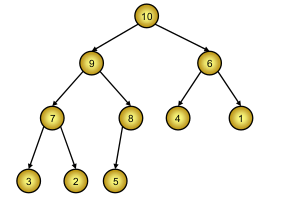
\includegraphics[scale=1]{img/heaptree.png}
\caption{Heap}
\label{HeapTree}
\end{figure}

\subsubsection{Vun đống}

Để biểu diễn dãy khóa arr[0...len-1] thành một cây nhị phân hoàn chỉnh. Giá trị arr[i] lưu trong nút thứ i (i bắt đầu từ 0). Nút con trái của nút thứ i là arr[2i+1] và con phải của nút thứ i là arr[2i+2]. Nút cha của nút thứ j là $(j-1) \% 2$.

Vì cây nhị phân gồm một nút thì hiển nhiên là đống. nên \textbf{để vun một nhánh cây gốc \texttt{r} thành đống, ta có thể coi hai nhánh con của nó là đống rồi và thực hiện thuật toán vun đống từ dưới lên đối với cây}. Gọi h là chiều cao của cây, nút ở mức h (nút lá) đã là một đống, ta vun lên những nút ở mức $h-1$ cũng là gốc của đống,... cứ như vậy cho tới mức 1 cũng là gốc của đống.

\paragraph{Thuật toán vun đống đối với gốc \texttt{r} khi hai nhánh con đã là đống}
Giả sử nút r chứa giá trị V. Tử r, ta cứ đi tới nút con chứa giá trị lớn nhất trong hai nút con, cho tới khi gặp phải một nút c mà mọi nút con của c đều có giá trị $ \le $ V (nút lá cũng là trường hợp riêng của điều kiện này). Dọc đường đi từ r tới c, ta đẩy giá trị chứa ở nút con lên nút cha và đặt giá trị V vào nút c.
\pagebreak 
\begin{figure}[htp]
\centering
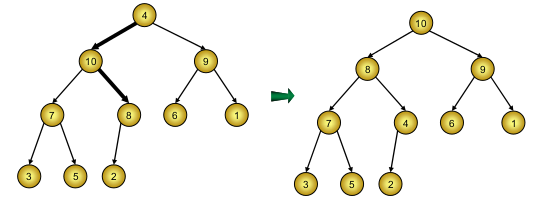
\includegraphics[scale=0.50]{img/buildheap.png}
\caption{Vun đống}
\label{}
\end{figure}

\subsubsection{Tư tưởng của Heap Sort}

Đầu tiên với dãy khóa arr[0...len-1] được vun từ dưới lên để nó biểu diễn một đống, khi đó khóa arr[0] tương ứng với nút gốc của đống là khóa lớn nhất, ta đảo giá trị khóa đó cho arr[len-1] và không tính tới arr[len-1] nữa. Còn lại dãy khóa arr[0...len-2] tuy không là đống nữa nhưng là biểu diễn của cây nhị phân hoàn chỉnh mà hai nhánh cây đã là đống rồi. Vậy chỉ cần vun một lần, ta lại dược một đống, đảo giá trị arr[0] với arr[len-2] rồi tiếp tục tới khi đống chỉ còn lại một nút.

\begin{figure}[htp]
\centering
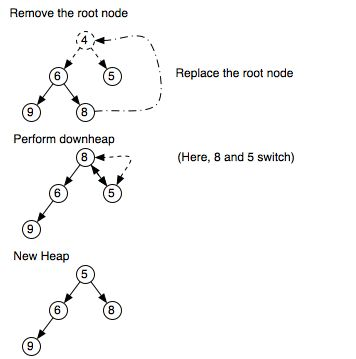
\includegraphics[scale=0.5]{img/tachdong.jpg}
\caption{Đảo giá trị của arr[0] và arr[len-1] rồi xét lại}
\label{}
\end{figure}

Thuật toán Heap Sort có hai hàm chính:

\begin{itemize}
\item Hàm \texttt{maxHeapify} làm nhiệm vụ vun cây gốc root thành đống trong điều kiện hai gốc con $2*root+1$ và $2*root+2$ đã là đống rồi. Các nút từ endnode+1 tới len-1 đã nằm đúng vị trí, không được tính tới nữa.
\item Hàm \texttt{heapSort} mô tả lại quá trình vun đống theo ý tưởng trên
\end{itemize}
\pagebreak
\mnt{src/heapsort.cpp}
































\end{document}